\chapter{Discussion}
\label{chap:discussion}

Intro discussion ? Poor performance?

\section{overfitting}

A recurring problem for the models trained for this thesis is the number of predictions that are identical to a label found in the training set.
When this occurs, it shows that a model is not able to achieve the task of predicting a de novo molecular representation from \ac{MS/MS}, but only repeats the data is has been trained with.
There are a few contributing factors to this overfitting problem with the setup used in this thesis.

\begin{description}
    \item[Duplicate training labels]
            As mentioned in the paper from MassSpecGym \cite{bushuiev2024massspecgym}, the dataset is a collection of the most qualitative annotated open-source mass spectrometry datasets.
            Even though a lot of filtering was performed after thorough quality control, the amount of duplicate molecules is significant.
            Figure \ref{fig:duplicate_smiles} shows the amount of SMILES that have multiple occurrences in the training set. Notice the logarithmic y-axis for readability.
            Even though 84\% of unique molecules have 10 occurrences or less, some molecules are noticeably more present in the training set, with one molecule being present 477 times in the training set.
            This imbalance does not necessarily reflect the real-world imbalance of molecules as it is caused by the use of imbalanced datasets.
            This causes the models to be trained with a bias towards these more frequent occurring molecules in the training set.
            This imbalance is also present in the validation (and test) set, where the most frequently occurring molecule accounts for 2.7\% (out of the almost 20.000 entries) of the validation data.
            Because of this imbalance, the models will be evaluated with a bias towards these more abundant molecules.
    \begin{figure}[h]
        \centering
        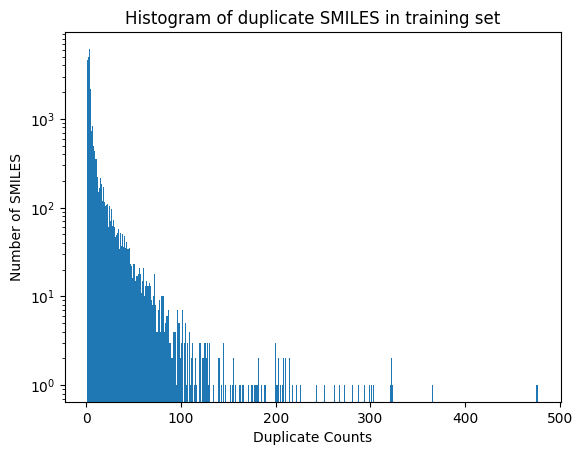
\includegraphics[width=0.6\textwidth]{figures/discussion/duplicate_smiles_training_set.png}
        \caption{distribution of duplicate SMILES in MassSpecGym's training set with a logarithmic scale}.
        \label{fig:duplicate_smiles}
    \end{figure}

    \item[Exposure bias] During training, a teacher forcing approach is used, where only the ground truth tokens are used to generate the next token iteratively.
    At inference time, when the model is sampled, the model does not get this help and has to rely on its own previous (incorrect) predictions.
    This is often referred to as exposure bias \cite{schmidt2019generalization}.
    The previously discussed imbalance of the training set only makes this bias worse, by training on these frequently occurring token combinations.
    This severely hinders the generalization of the model.
    An example of this exposure bias can be clearly seen in the results from the hyperparameter gridsearch (figure \ref{fig:gridsearch_vs_paper}), where a model with a lower validation loss performed worse at inference time.
    The loss has this teacher forced advantage, while the metrics calculated on the sampled predictions do not.
    Because all models trained in this thesis are optimized for validation loss, it can be questioned if they have been overfit on these teacher forced predictions.
    
    \item[Evaluation metrics] The metric that best describes how close close a prediction is to the actual molecule is the \ac{MCES} distance.
    Problem: Does not show overfitting, even empty predictions can have low MCES distance...
\end{description}






%\section{Retraining MassSpecGym}
- loss function not optimal to determine model performance
- The SMILES validity is something the loss function can not measure.

overfitting:
    - dataset labels unbalanced
    - MCES distance does not show overfitting
    - teacher forcing + loss does not allow the model to predict synonym smiles




\section{Experiments}

SMILES veel overfitting, invloed op experimenten?

\subsection{Samplers benchmark}

- Beam search: Score function using loss is not optimal
\subsection{\ac{BPE} as pretraining}


\subsection{Augmentation}
Only BPE encoded SMILES models, overfitting might influence results

\subsection{SMILES augmentation}
- SMILES from molecular graph is deterministic, evaluation is done on only these deterministic outputs, by randomizing the SMILES with synonyms it confuses the model and will perform worse on the evaluated SMILES.
- model not powerfull enough
- BPE does not help because augmented patterns use more tokens
- less augmentation

\subsection{Spectral augmentation}

Could be used to fix mulecule imbalance, where only the least occurring molecules in the training set are augmented


\subsection{Molecular representations benchmark}

Models not optimized for hyperparameters
samplers chosen based of SMILES results

3 headed inchi could be improved by supplying the output of the previous decoder to the next, to ensure they know what molecule it is trying to predict

SELFIES can benefit from BPE because some tokens have different meaning in context of rings and groups, without the model overfitting

\section{Future for de novo structure prediction}

- string based representations not suited, reference graph based paper
- autoregressive models not suited for molecular structure generation by exposure bias